%\documentclass[dvipdfmx,fleqn]{beamer}
\documentclass[dvipdfmx,fleqn,handout]{beamer}
\usepackage{amsmath,amssymb,amsthm}

\mode<presentation>
{
  \usetheme{default}
}

\title{\Large Fictitious play}
\author{\large 花嶋 陽}
\date{\small 6/28}

\usefonttheme{professionalfonts}

\setbeamercovered{transparent=20}

\setbeamertemplate{navigation symbols}{} 
\setbeamertemplate{footline}[frame number] 



\begin{document}

\sffamily
\gtfamily


\begin{frame}
  \titlepage
  \thispagestyle{empty}
\end{frame}

\setcounter{framenumber}{0}




\begin{frame}
\frametitle{はじめに}
\begin{itemize}\setlength{\parskip}{0.5em}
\item
項目1

\item
項目2
 \begin{itemize}\setlength{\parskip}{0.5em}
 \item
 1階層下の項目1
 \item
 1階層下の項目2
 \end{itemize}

\item
このページの最後の項目
\end{itemize}
\end{frame}



\begin{frame}
\frametitle{次のスライド}
\begin{itemize}\setlength{\parskip}{0.5em}
\item
Ficititious playの説明1

\item
Ficititious playの説明2 \pause

$x_0(t)$ は
\[
x_0(t+1)
= x_0(t) + \frac{1}{t+2} (a_1(t) - x_0(t))
\]
と再帰的に書くことができる. \pause

\item
Ficititious playの説明3 \pause

\item
``\texttt{pause}''をつけるとoverlayができる.

\item
ファイルの冒頭の\texttt{documentclass}のオプションで\texttt{handout}を指定すると,
overlayにならずいっぺんに表示される.

Webにのせるときや,印刷して配るときなどは\texttt{handout}を指定しておく.

\end{itemize}
\end{frame}



\begin{frame}[containsverbatim]% verbatim 環境を使えるように
\frametitle{コードの説明}
\begin{itemize}\setlength{\parskip}{0.5em}
\item
コードの内容
\begin{verbatim}
# -*- coding: utf-8 -*-
from __future__ import division  
import matplotlib.pyplot as plt
from random import uniform, choice
import numpy as np

def fictplay(t):
    x_0_t = [uniform(0, 1)]
    x_1_t = [uniform(0, 1)]
    gain_0 = np.array([[1, -1], [-1, 1]])   #player0
    gain_1 = np.array([[-1, 1], [1, -1]])   #player1
\end{verbatim}

\end{itemize}
\end{frame}

\begin{frame}[containsverbatim]% verbatim 環境を使えるように
\frametitle{コードの説明}
\begin{verbatim}
   for i in range(t):
        pro_1 = np.array([1-x_0_t[i], x_0_t[i]])      
		         #probability: player1 choice 0 or 1
         
     exp_gain_0 = np.dot(gain_0, pro_1)            
        #expected gain = gain × probability
        
     if exp_gain_0[0] > exp_gain_0[1]:
            a_0_i = 0
        elif exp_gain_0[0] == exp_gain_0[1]:
            a_0_i = choice([0, 1])
        else:
            a_0_i = 1

\end{verbatim}

\end{frame}

\begin{frame}[containsverbatim]% verbatim 環境を使えるように
\frametitle{コードの説明}
\begin{verbatim}
        pro_0 = np.array([1-x_1_t[i], x_1_t[i]])   
        exp_gain_1 = np.dot(gain_1, pro_0)
        if exp_gain_1[0] > exp_gain_1[1]:
            a_1_i = 0
        elif exp_gain_1[0] == exp_gain_1[1]:
            a_1_i = choice([0, 1])
        else:
            a_1_i = 1
        
        x_0_i1 = x_0_t[i] + (a_1_i - x_0_t[i]) / (i+2)
        x_1_i1 = x_1_t[i] + (a_0_i - x_1_t[i]) / (i+2)
        x_0_t.append(x_0_i1)
        x_1_t.append(x_1_i1)

    return x_0_t, x_1_t

\end{verbatim}

\end{frame}

\begin{frame}[containsverbatim]% verbatim 環境を使えるように
\frametitle{コードの説明}

\begin{verbatim}
x_0_t, x_1_t = fictplay(1000)
         
plt.plot(x_0_t, 'r-', label="x_0(t)")
plt.plot(x_1_t, 'b-', label="x_1(t)")
plt.legend()
#plt.savefig('fictplay0.png')
plt.show()

#x_0_t = []
#for i in range(100):
#    x_0, x_1 = fictplay(100)
#    x_0_t.append(x_0[-1])
#plt.hist(x_0_t)
#plt.savefig('fictplay_hist.png')
#plt.show()
\end{verbatim}


\end{frame}

\begin{frame}[containsverbatim]% verbatim 環境を使えるように
\frametitle{コードの説明}
\begin{itemize}\setlength{\parskip}{0.5em}
\item
コードの内容
\begin{verbatim}
\verb|\begin{frame}| から \verb|\end{frame}| までを
コピー\&ペーストしてスライドを増やしていく.
\end{verbatim}

\end{itemize}
\end{frame}


\begin{frame}
\frametitle{図}
\begin{figure}
 \centering
 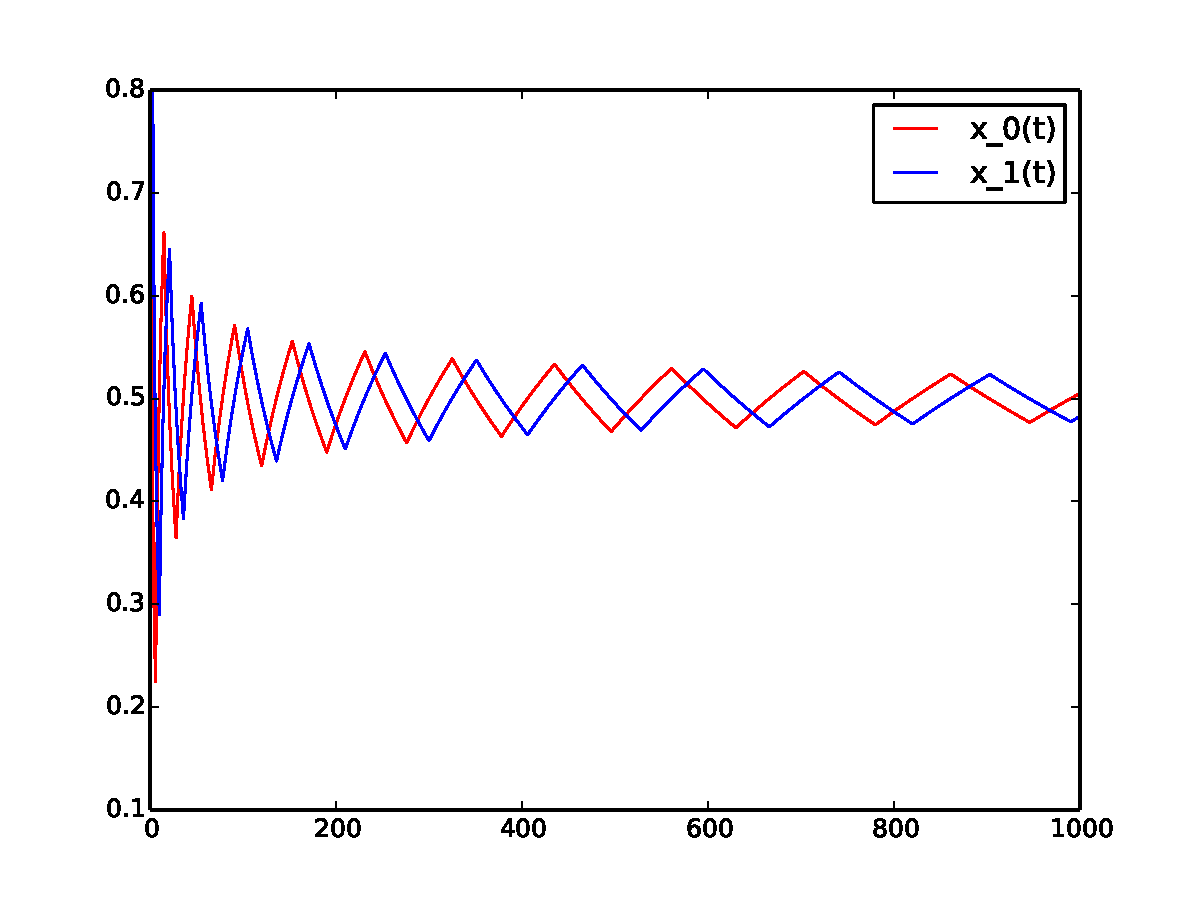
\includegraphics[scale=0.5]{matchingpennies_plot.pdf}
 \caption{図の表示}
 \label{fig:matchingpennies_plot}
\end{figure}
\end{frame}



\begin{frame}
\frametitle{まとめ}
\begin{itemize}\setlength{\parskip}{0.5em}
\item
まとめ

\item
よくわかっていない点とか

\item
今後の課題とか
\end{itemize}
\end{frame}



\end{document}